\documentclass{article}
\usepackage[margin=1in]{geometry}
\usepackage{amsmath,amsthm,amssymb}
\usepackage{bbm,enumerate,mathtools}
\usepackage{tikz,pgfplots}
\usepackage{chessboard}
\usepackage[hidelinks]{hyperref}
\usepackage{multicol} % Problem 35

\newenvironment{question}{\begin{trivlist}\item[\textbf{Question.}]}{\end{trivlist}}
\newenvironment{note}{\begin{trivlist}\item[\textbf{Note.}]}{\end{trivlist}}
\newenvironment{references}{\begin{trivlist}\item[\textbf{References.}]}{\end{trivlist}}
\newenvironment{related}{\begin{trivlist}\item[\textbf{Related.}]\end{trivlist}\begin{enumerate}}{\end{enumerate}}


\begin{document}
\rating{2}{1}
Consider dynamical billiards where the length of paths is given by some sequence.
% OutgoingArrow[incoming_Arrow,boundary_InfiniteLine,lineLength_]:=Module[{p1,p2,q1,q2,v},
% {p1,p2}=Identity@@incoming;
% {q1,q2}=Identity@@boundary;
% v=Projection[p2-p1,q2-q1];
% Arrow[{p2,p2+lineLength (p1+2v-p2)/Norm[p1+2v-p2]}]
% ]
% SeedRandom[56];
% a1=Arrow[{{0,0},{0,3}}];
% b1=InfiniteLine[{{0,3},RandomReal[{-10,10},2]}];
% a2=OutgoingArrow[a1,b1,1]//N;
% b2=InfiniteLine[{a2[[1,2]],RandomReal[{-10,10},2]}]//N;
% a3=OutgoingArrow[a2,b2,4];
% b3=InfiniteLine[{a3[[1,2]],RandomReal[{-10,10},2]}]//N;
% a4=OutgoingArrow[a3,b3,1];
% b4=InfiniteLine[{a4[[1,2]],RandomReal[{-10,10},2]}]//N;
% a5=OutgoingArrow[a4,b4,5];
% b5=InfiniteLine[{a5[[1,2]],RandomReal[{-10,10},2]}]//N;
% a6=OutgoingArrow[a5,b5,9];
% b6=InfiniteLine[{a6[[1,2]],RandomReal[{-10,10},2]}]//N;
% Graphics[
%   {
%     a1,a2,a3,a4,a5,
%     Dashed,Red,
%     b1,b2,b3,b4,b5,
%     Nothing
%   },
%   PlotRange->{{-3,3},{-1,5}},AspectRatio->1
% ]
\begin{figure}[ht!]
  \[
  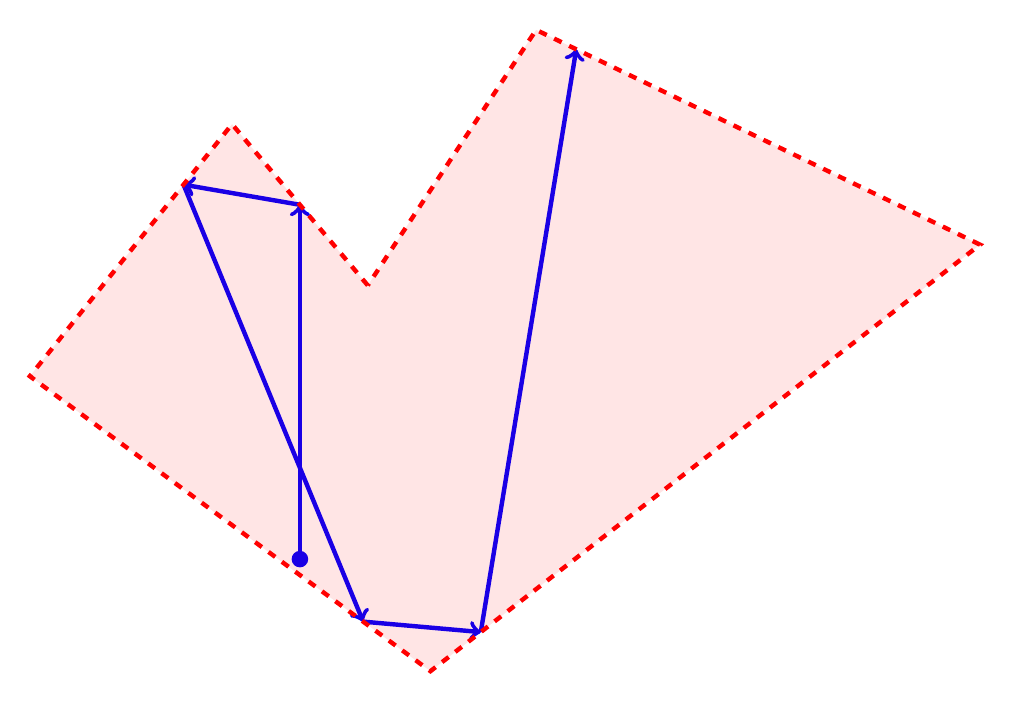
\begin{tikzpicture}[scale=1.5]
    \fill[blue] (0,0) circle (0.07);
    % \draw (-3,-1) rectangle (3,5);
    \draw[ultra thick, blue, ->] (0,0) -- (0,3);
    \draw[ultra thick, blue, ->] (0,3) -- (-0.985392, 3.1703);
    \draw[ultra thick, blue, ->] (-0.985392, 3.1703) -- (0.535414, -0.529314);
    \draw[ultra thick, blue, ->] (0.535414, -0.529314) -- (1.53149, -0.617783);
    \draw[ultra thick, blue, ->] (1.53149, -0.617783) -- (2.33959, 4.31648);
    \draw[ultra thick, red, dashed, fill=red, fill opacity=0.1]
      (0.574636,2.31753)--
      (0, 3)--
      (-0.574636, 3.68247)--
      (-2.28623, 1.5483)--
      (1.10503, -0.948726)--
      (5.75844, 2.66237)--
      (2.33959, 4.31648)--
      (2., 4.48078)--
      cycle;
  \end{tikzpicture}
  \]
  \caption{
    An example of a path for $(3,1,4,1,5)$
  }
\end{figure}

\begin{question}
  Given a sequence of lengths, can we describe a billiards table together with an initial position, and initial velocity that results in the given sequence of lengths?
\end{question}

\begin{related}
  \item Given a sequence of lengths, can we compute the smallest polygon by number of sides containing a corresponding billiards path?
  \item Does every sequence of lengths correspond to some convex billiards table?
  \item What if we want the path to form a cycle?
  \item What if we want the billiards path to be non-self-intersecting?
\end{related}

\begin{references}
  \item \url{https://www.instagram.com/p/CrYp3fTOPMu/}
\end{references}
\end{document}
